\newpage
\section{Результаты измерений}

\[V=800\pm5\,\text{см}^3\]
\[l/S=1500\pm 100\,\text{см}^{-1}\]



\begin{figure}
    \centering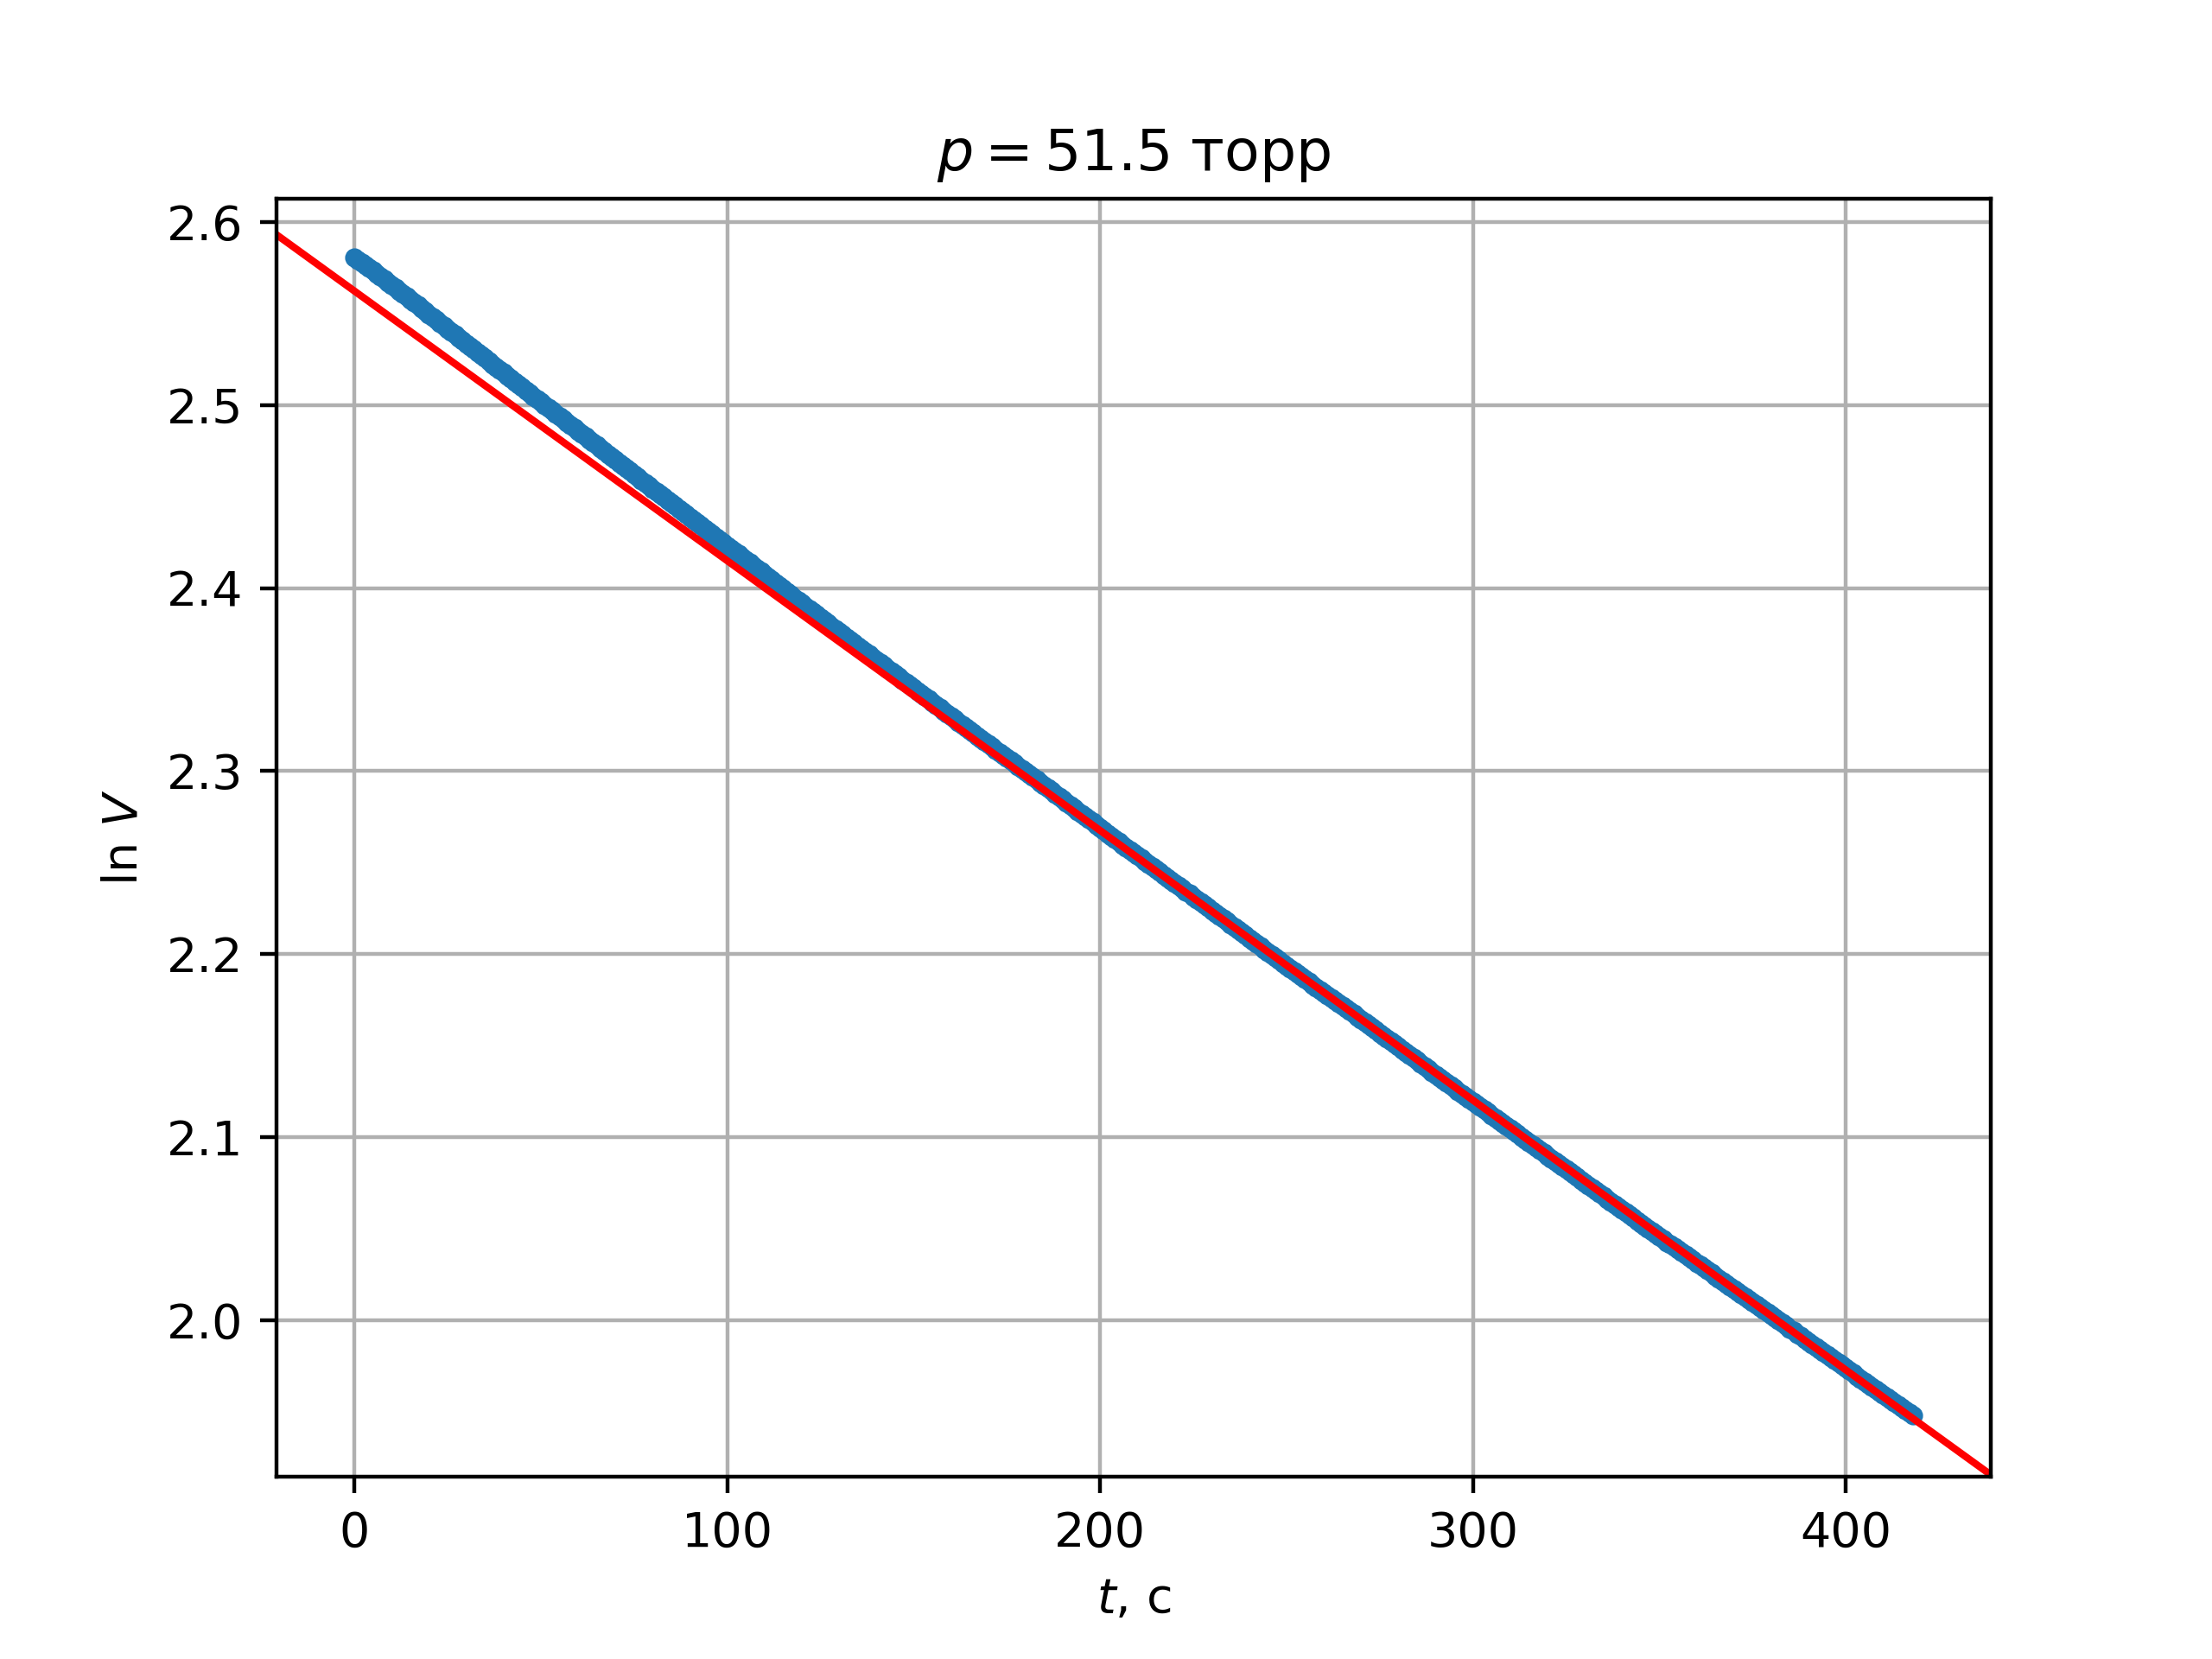
\includegraphics[width=0.45\linewidth]{img/data1.png}
    \centering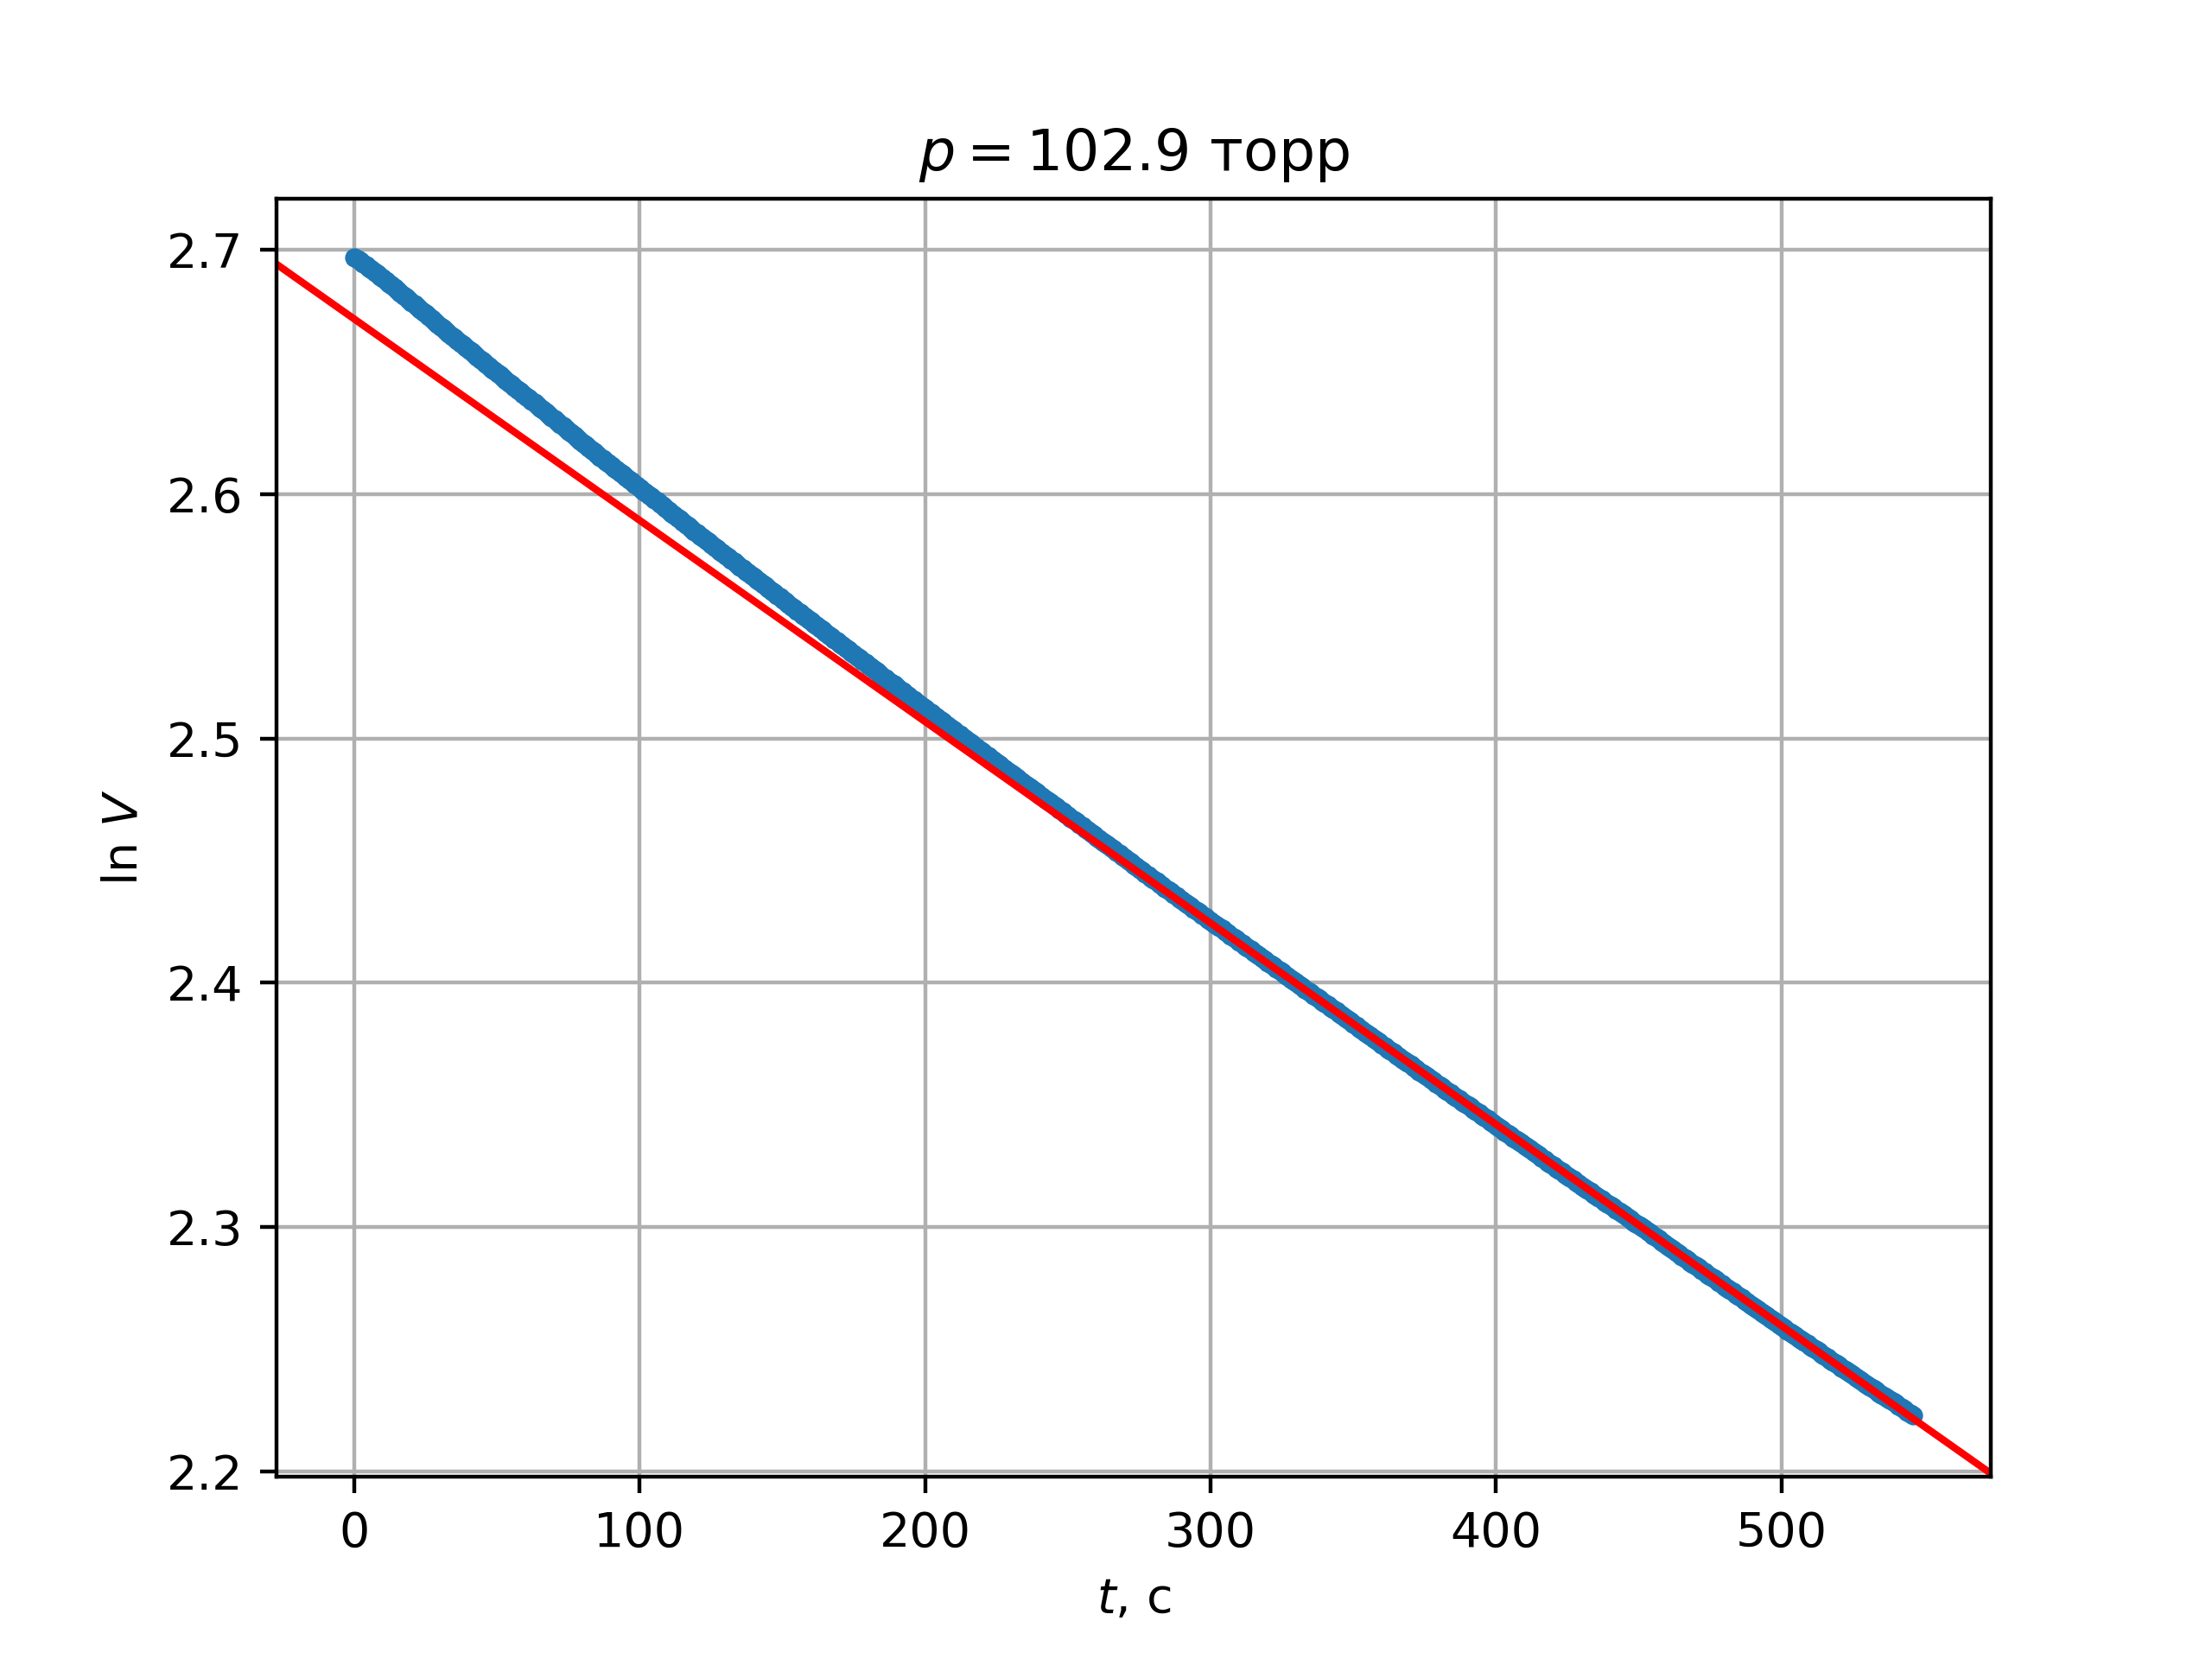
\includegraphics[width=0.45\linewidth]{img/data2.png}
    \centering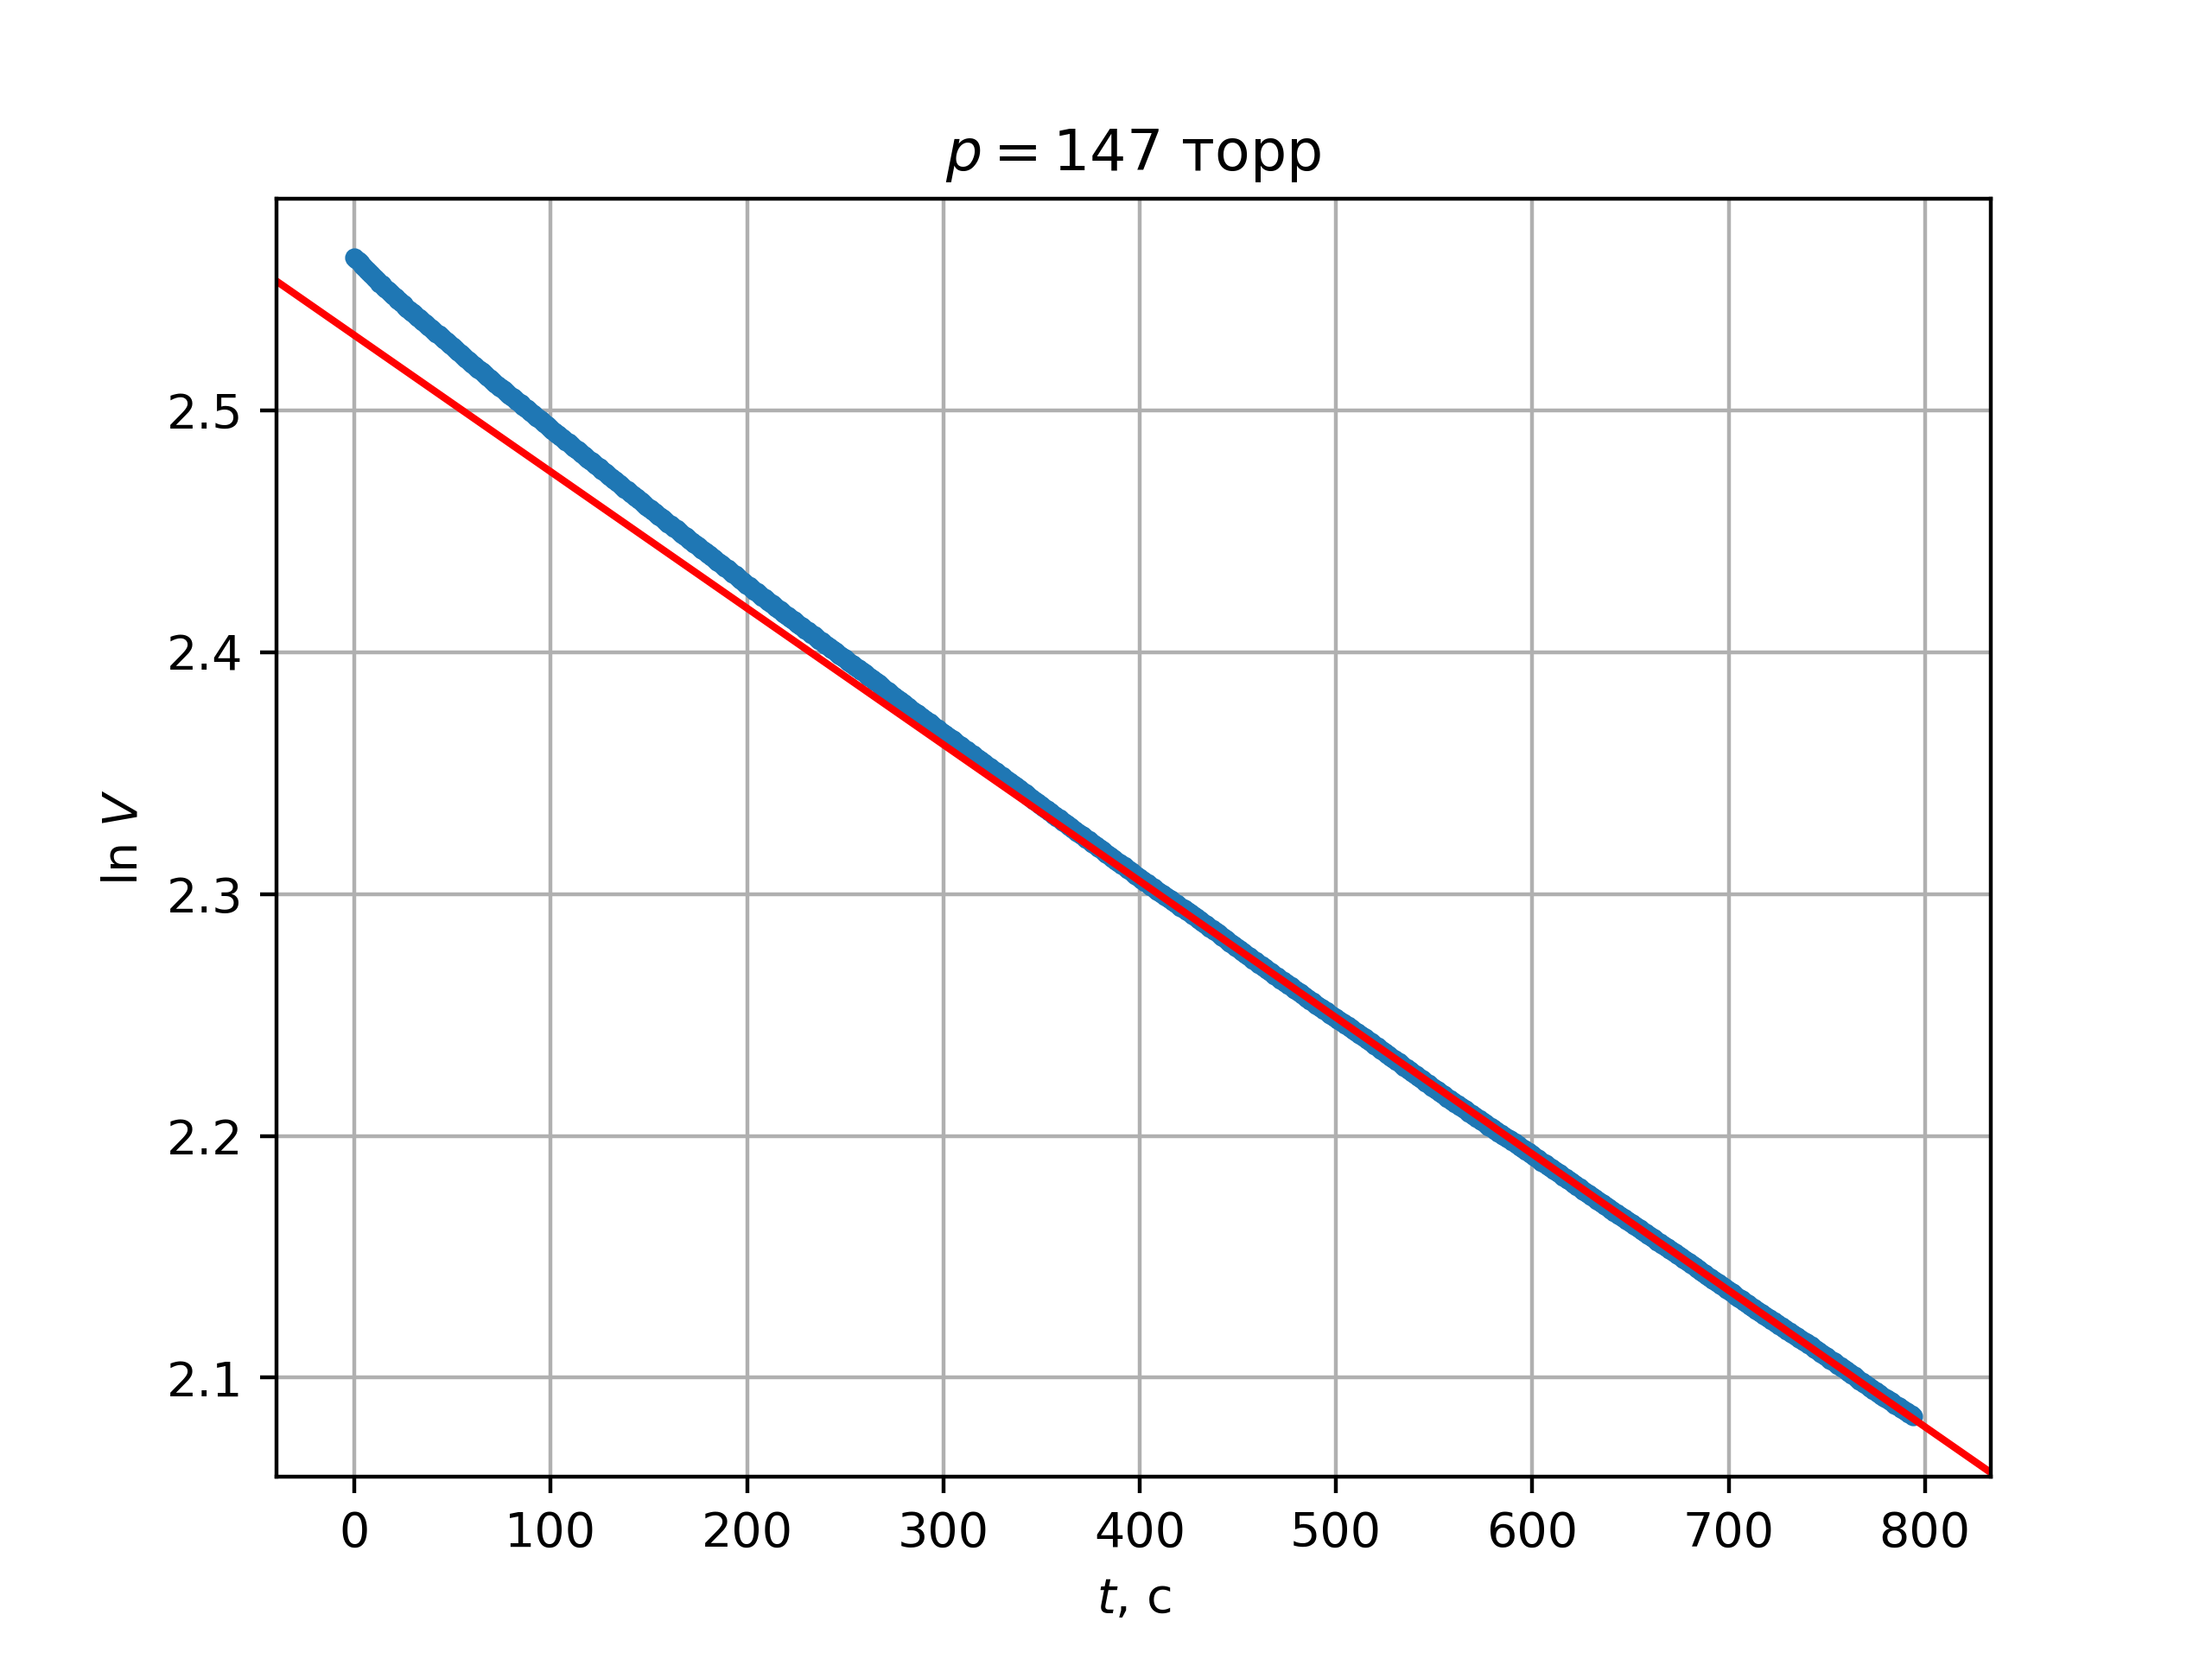
\includegraphics[width=0.45\linewidth]{img/data3.png}
    \centering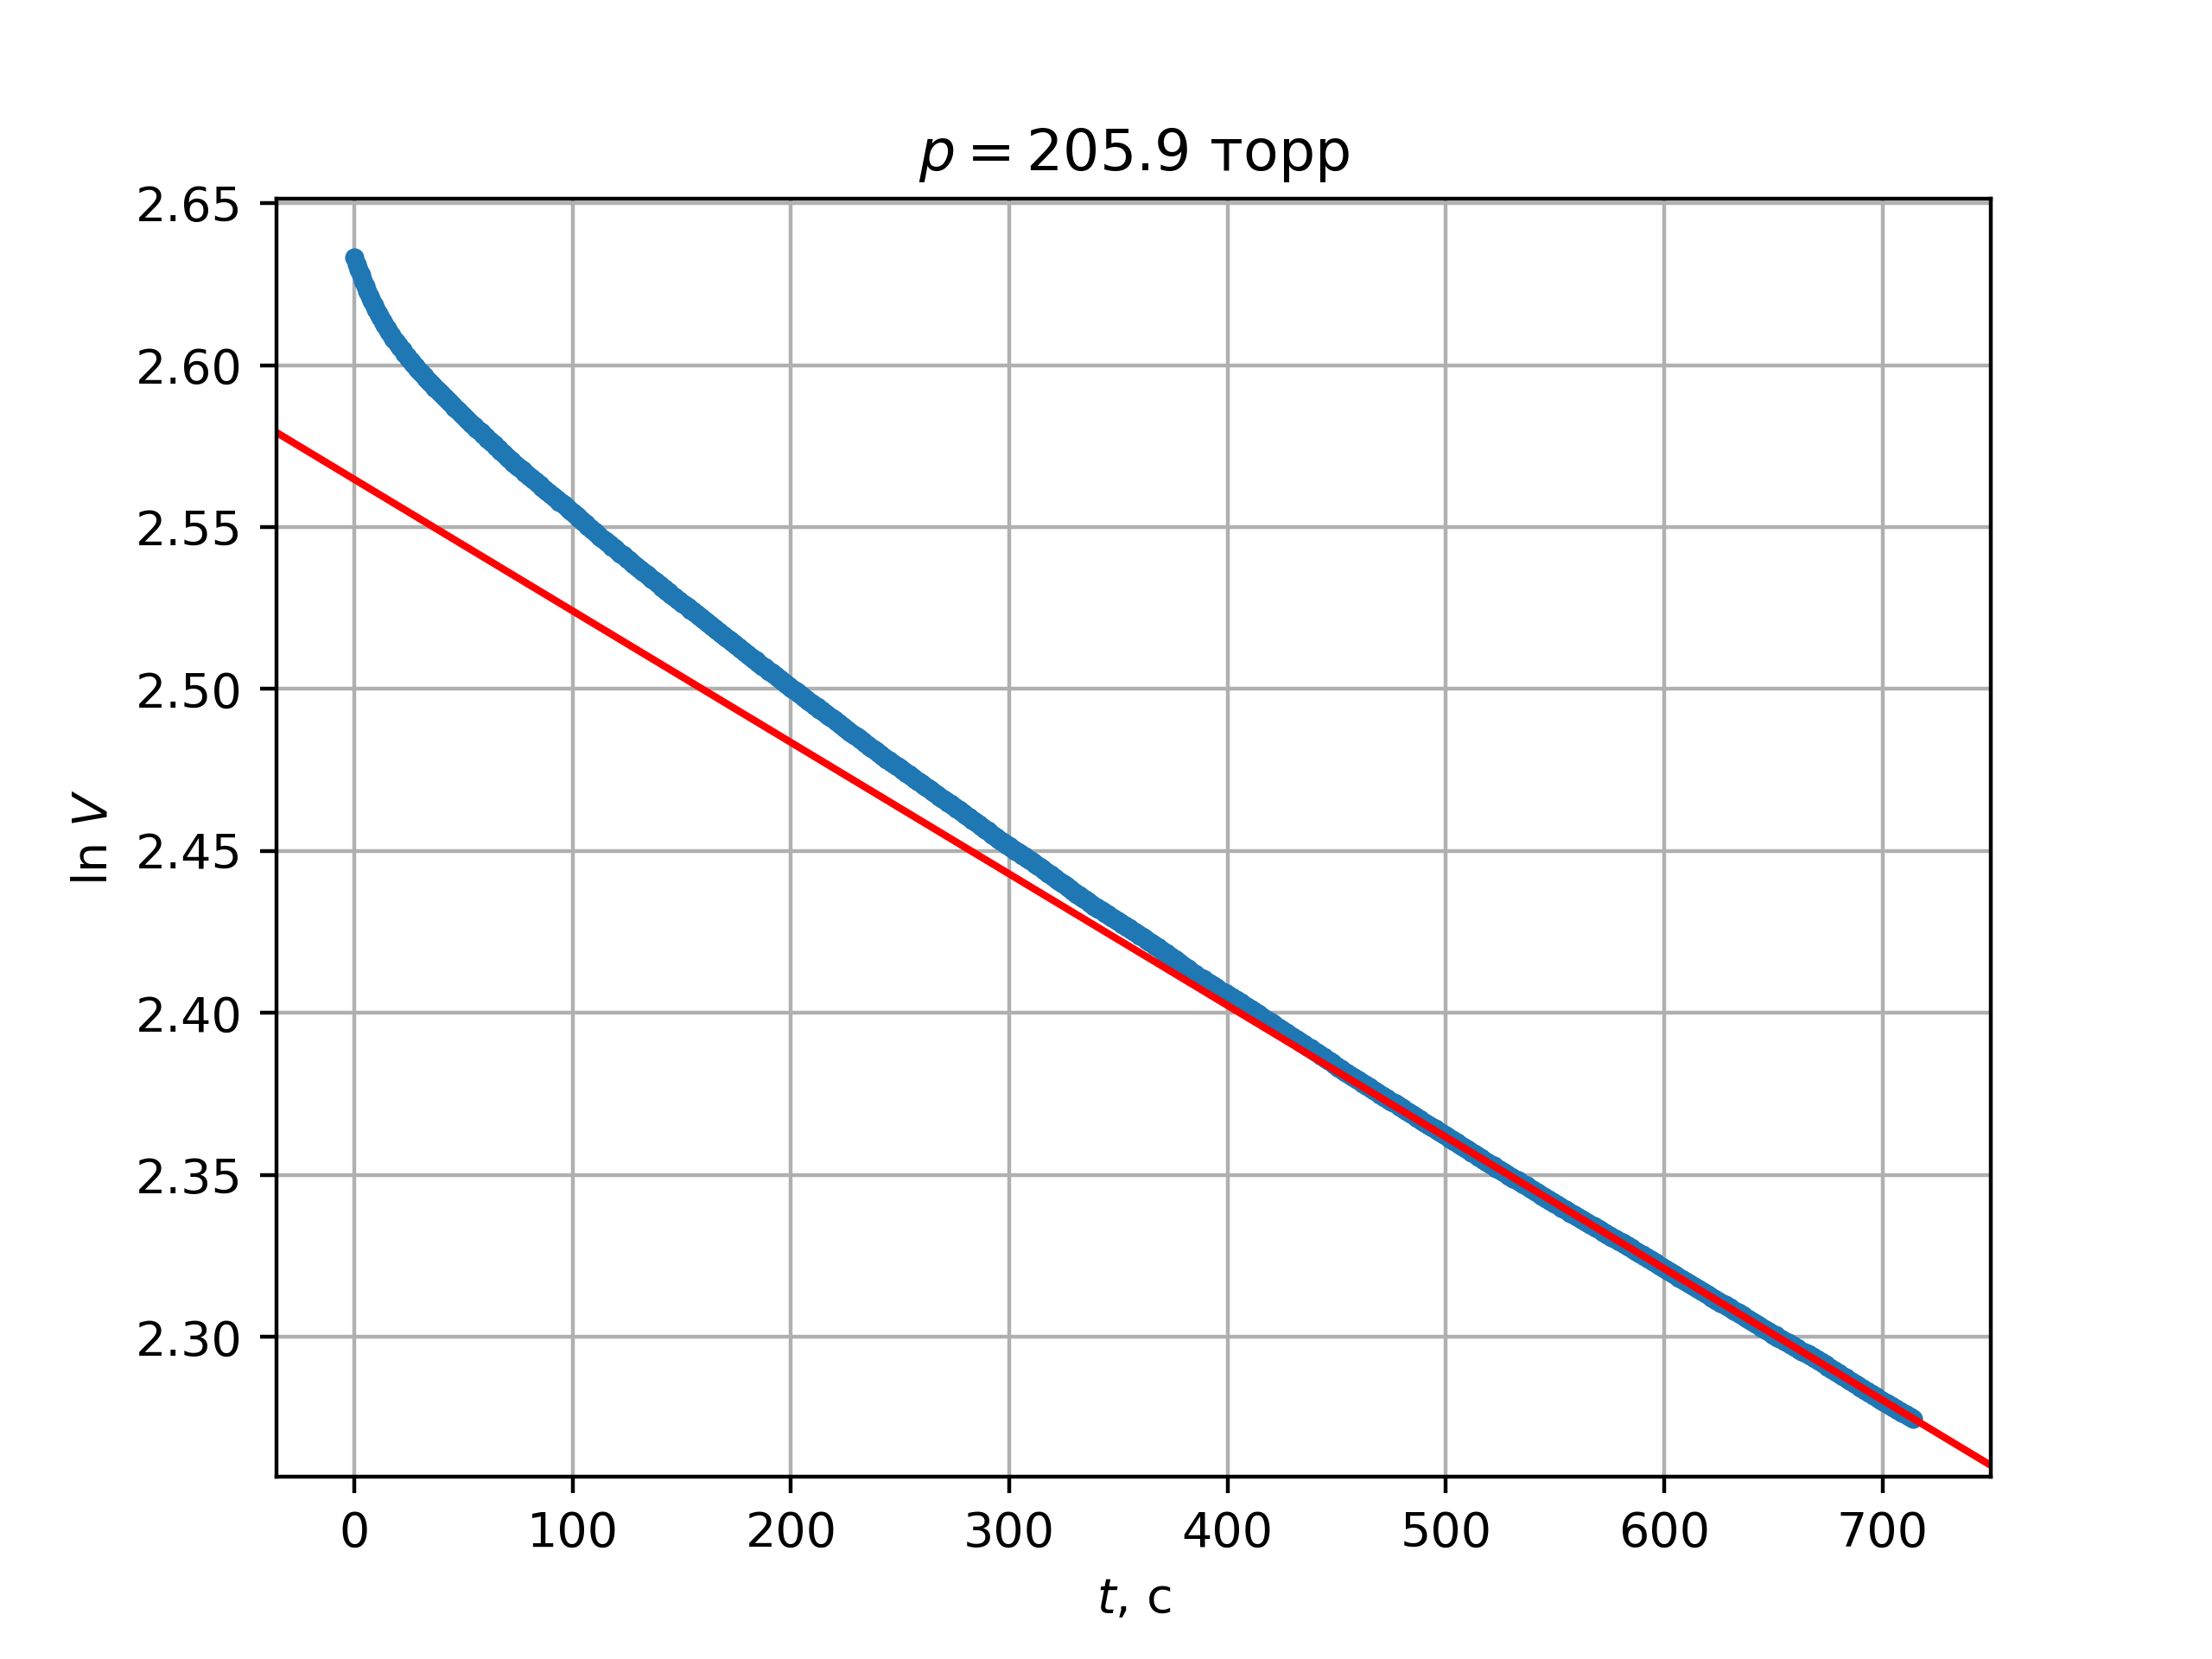
\includegraphics[width=0.45\linewidth]{img/data4.png}
    \centering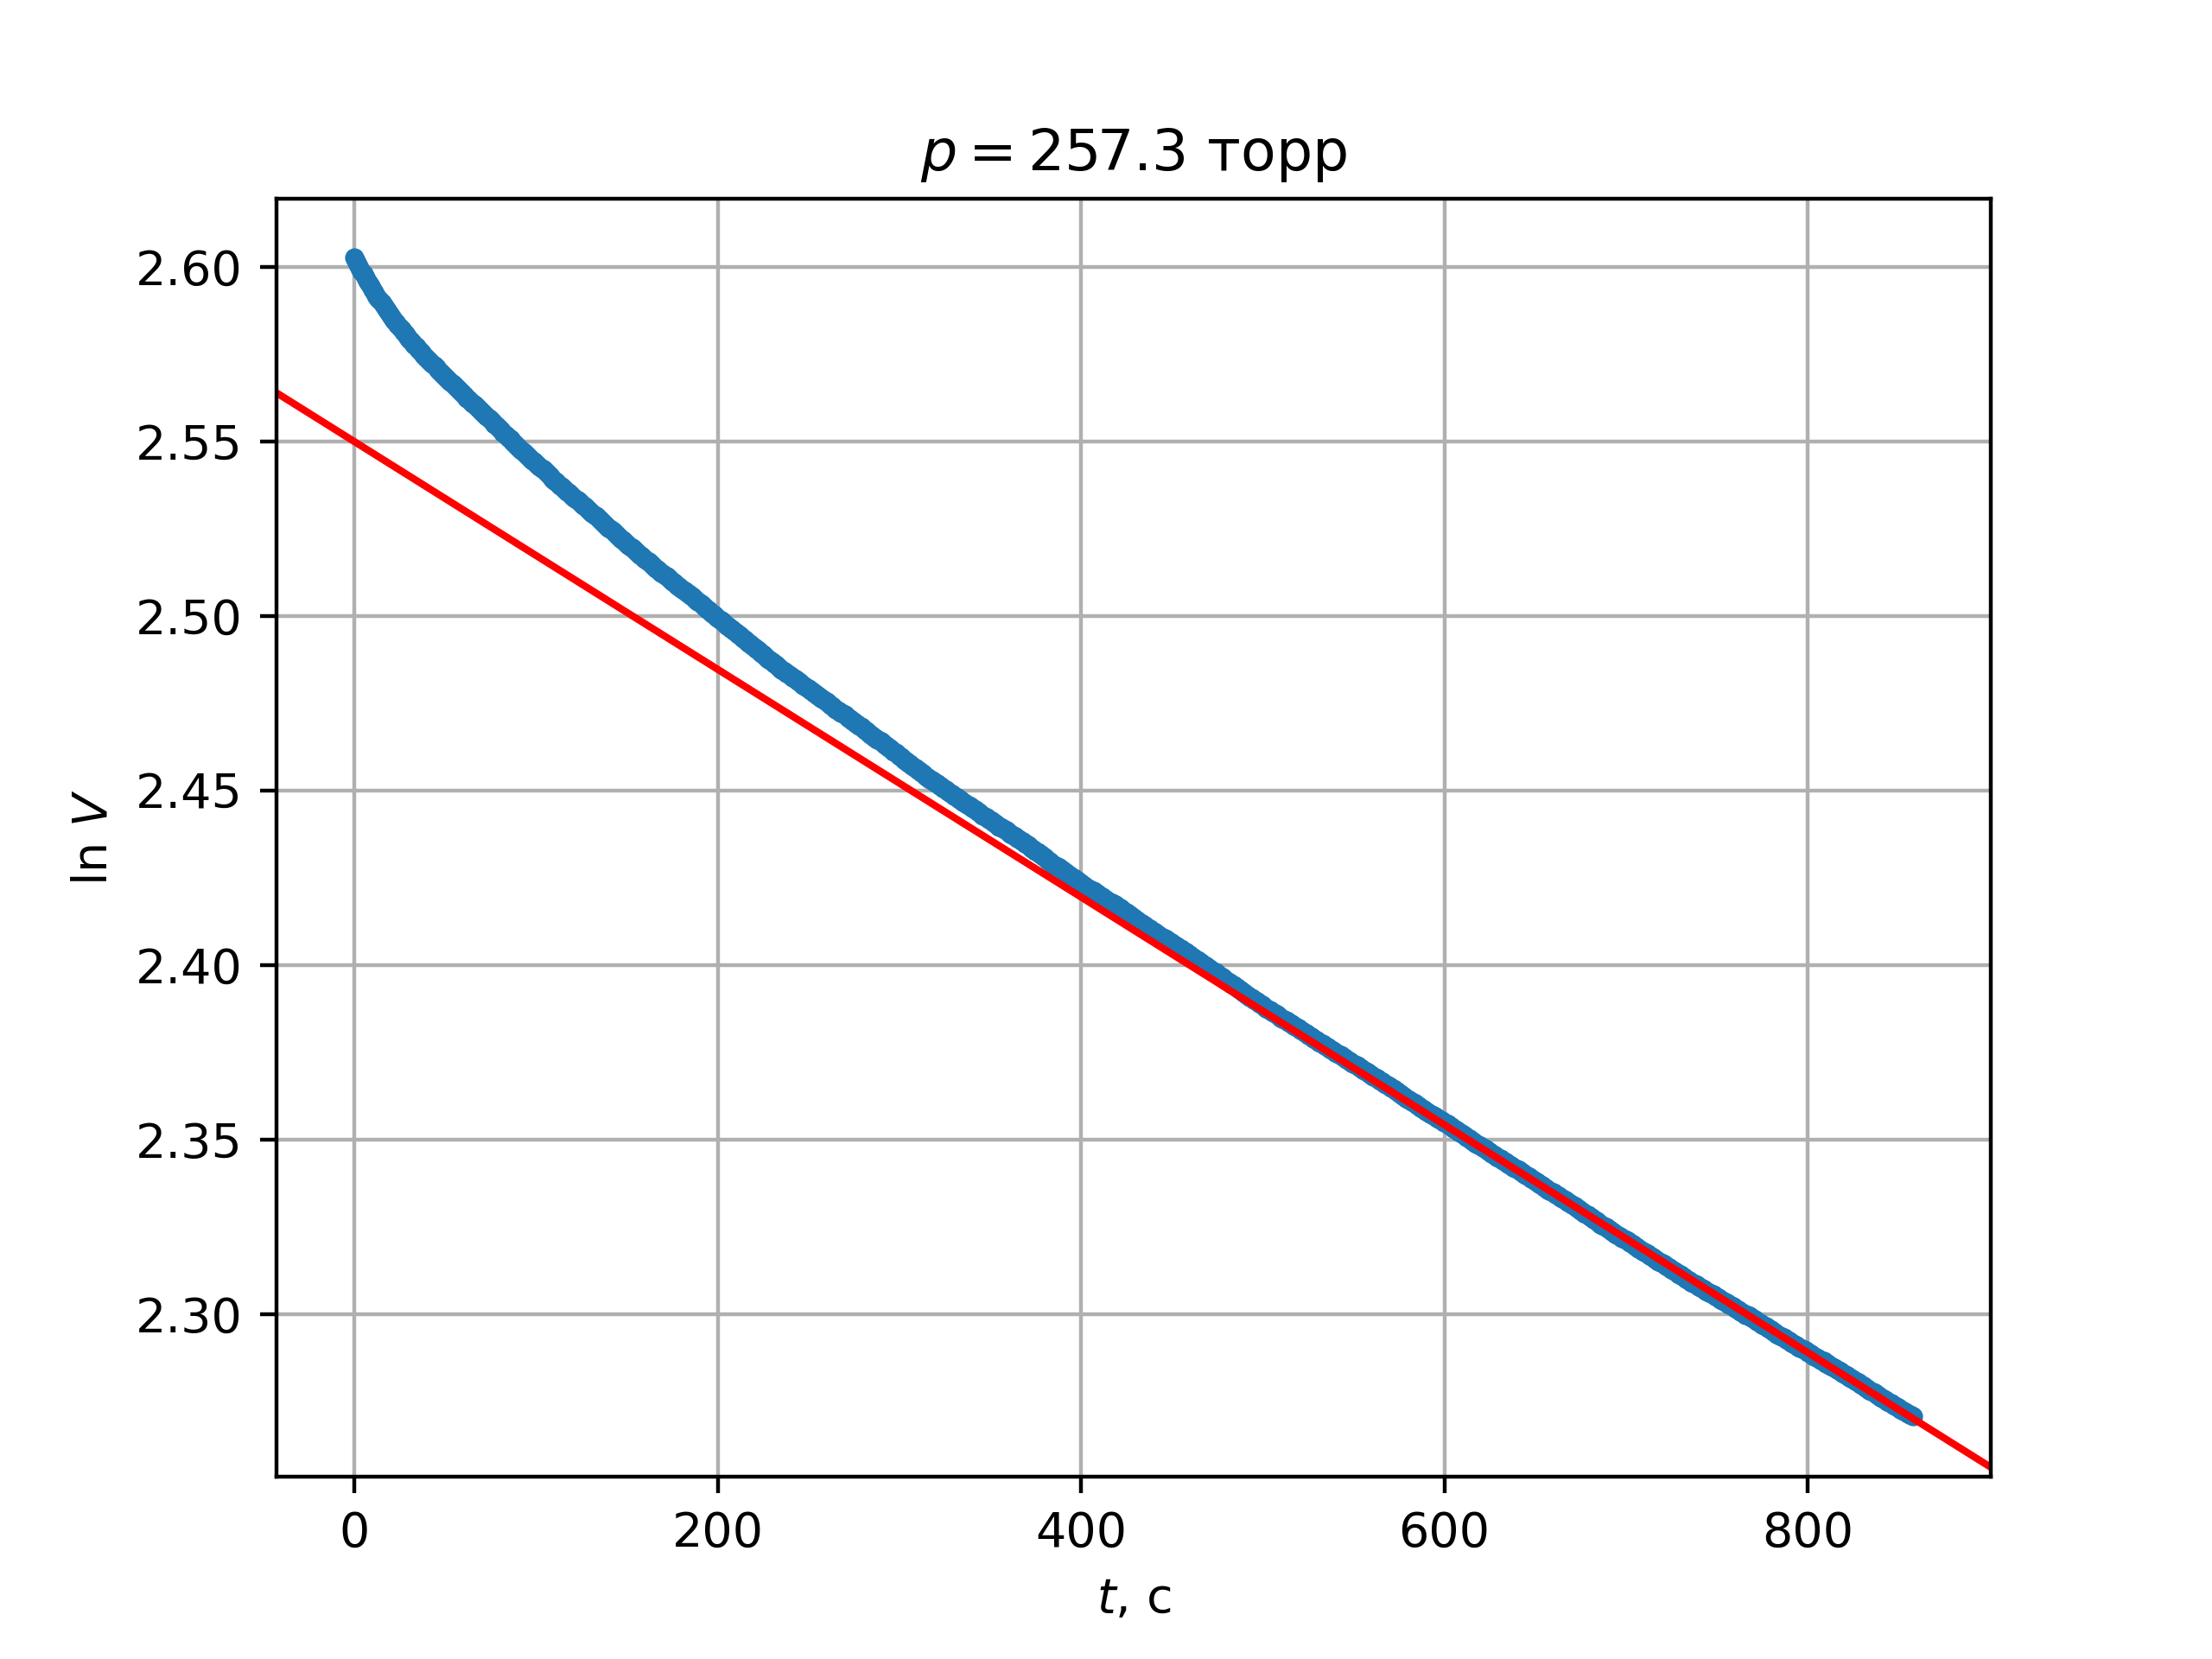
\includegraphics[width=0.45\linewidth]{img/data5.png}
    \centering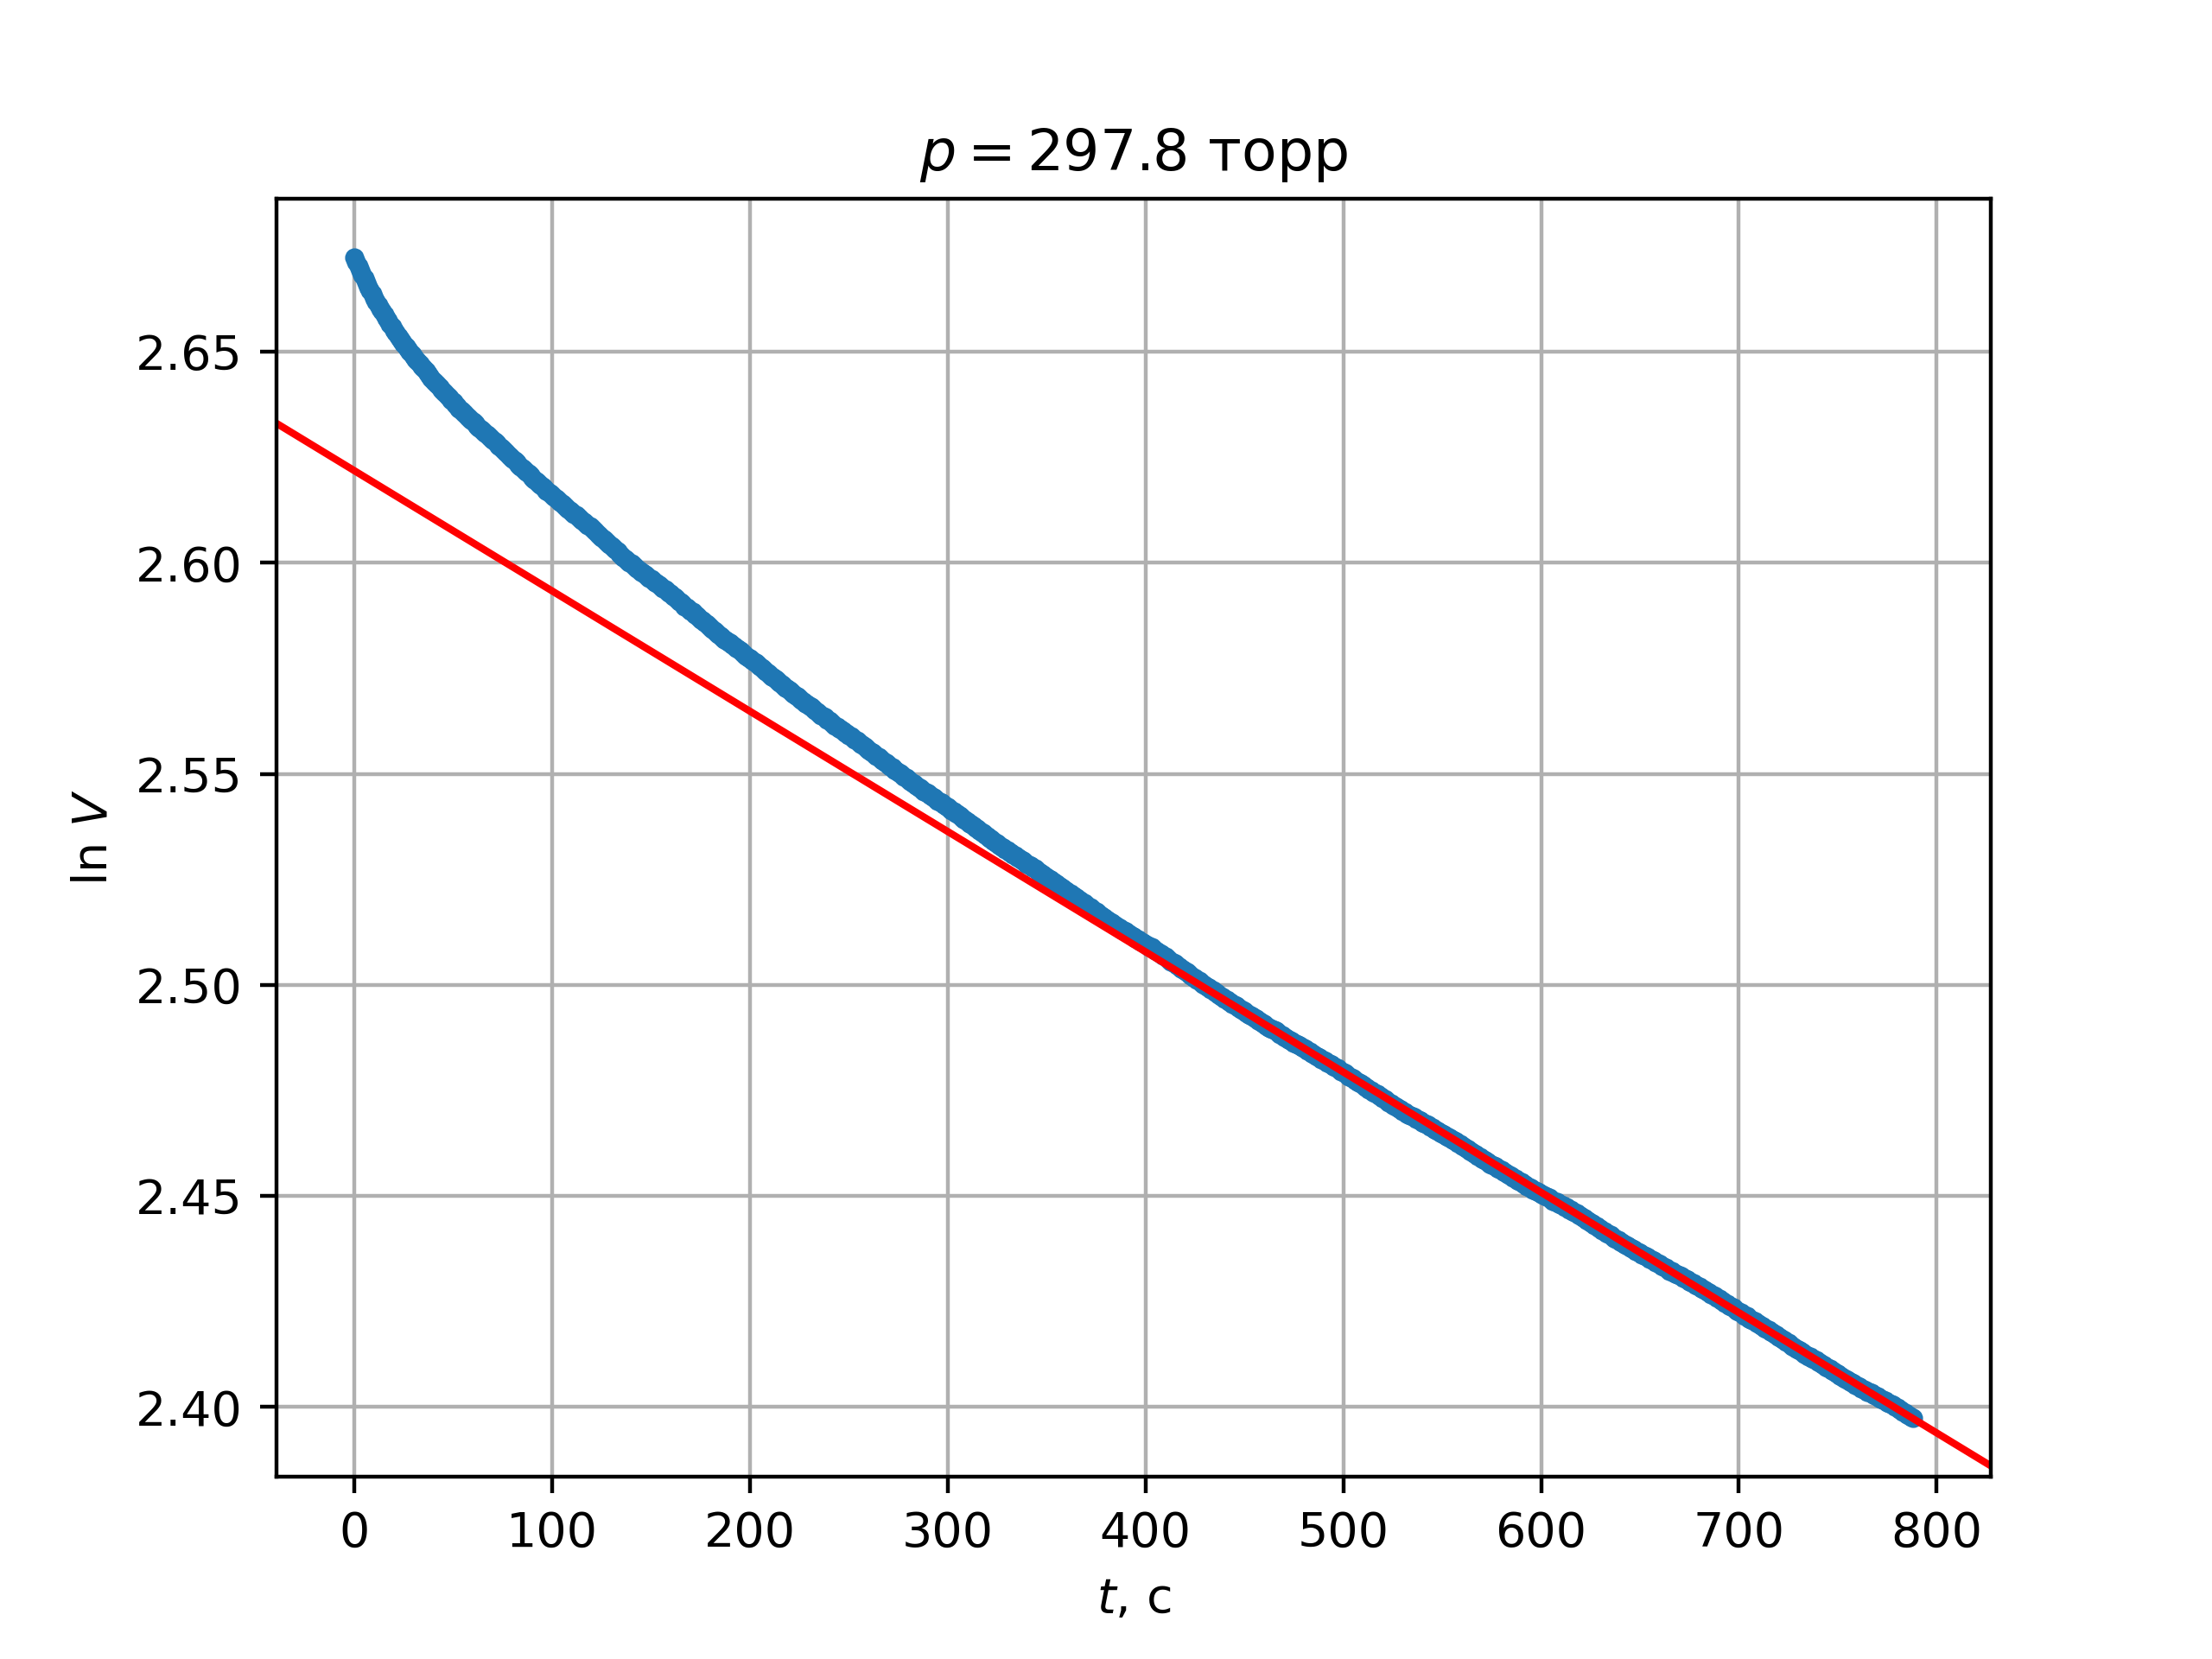
\includegraphics[width=0.45\linewidth]{img/data6.png}
\end{figure}

\begin{table}[]
    \begin{tabular}{|l|l|l|l|l|l|l|}
    \hline
    $D,\cdot 10^{-5}\,\text{м}^2/\text{с}$ & $8{,}8\pm 0{,}6$ & $4{,}9\pm 0{,}4$ & $3{,}4\pm 0{,}2$ & $2{,}4 \pm 0{,}2$ & $1{,}96\pm 0{,}14$ & $1.71\pm 0{,}12$ \\ \hline
    $p\pm 0{,}25,\,\text{торр}$            & $51{,}5$         & $102{,}9$        & $147$            & $205{,}9$         & $257{,}3$          & $297{,}8$        \\ \hline
    \end{tabular}
\end{table}

\begin{figure}
    \centering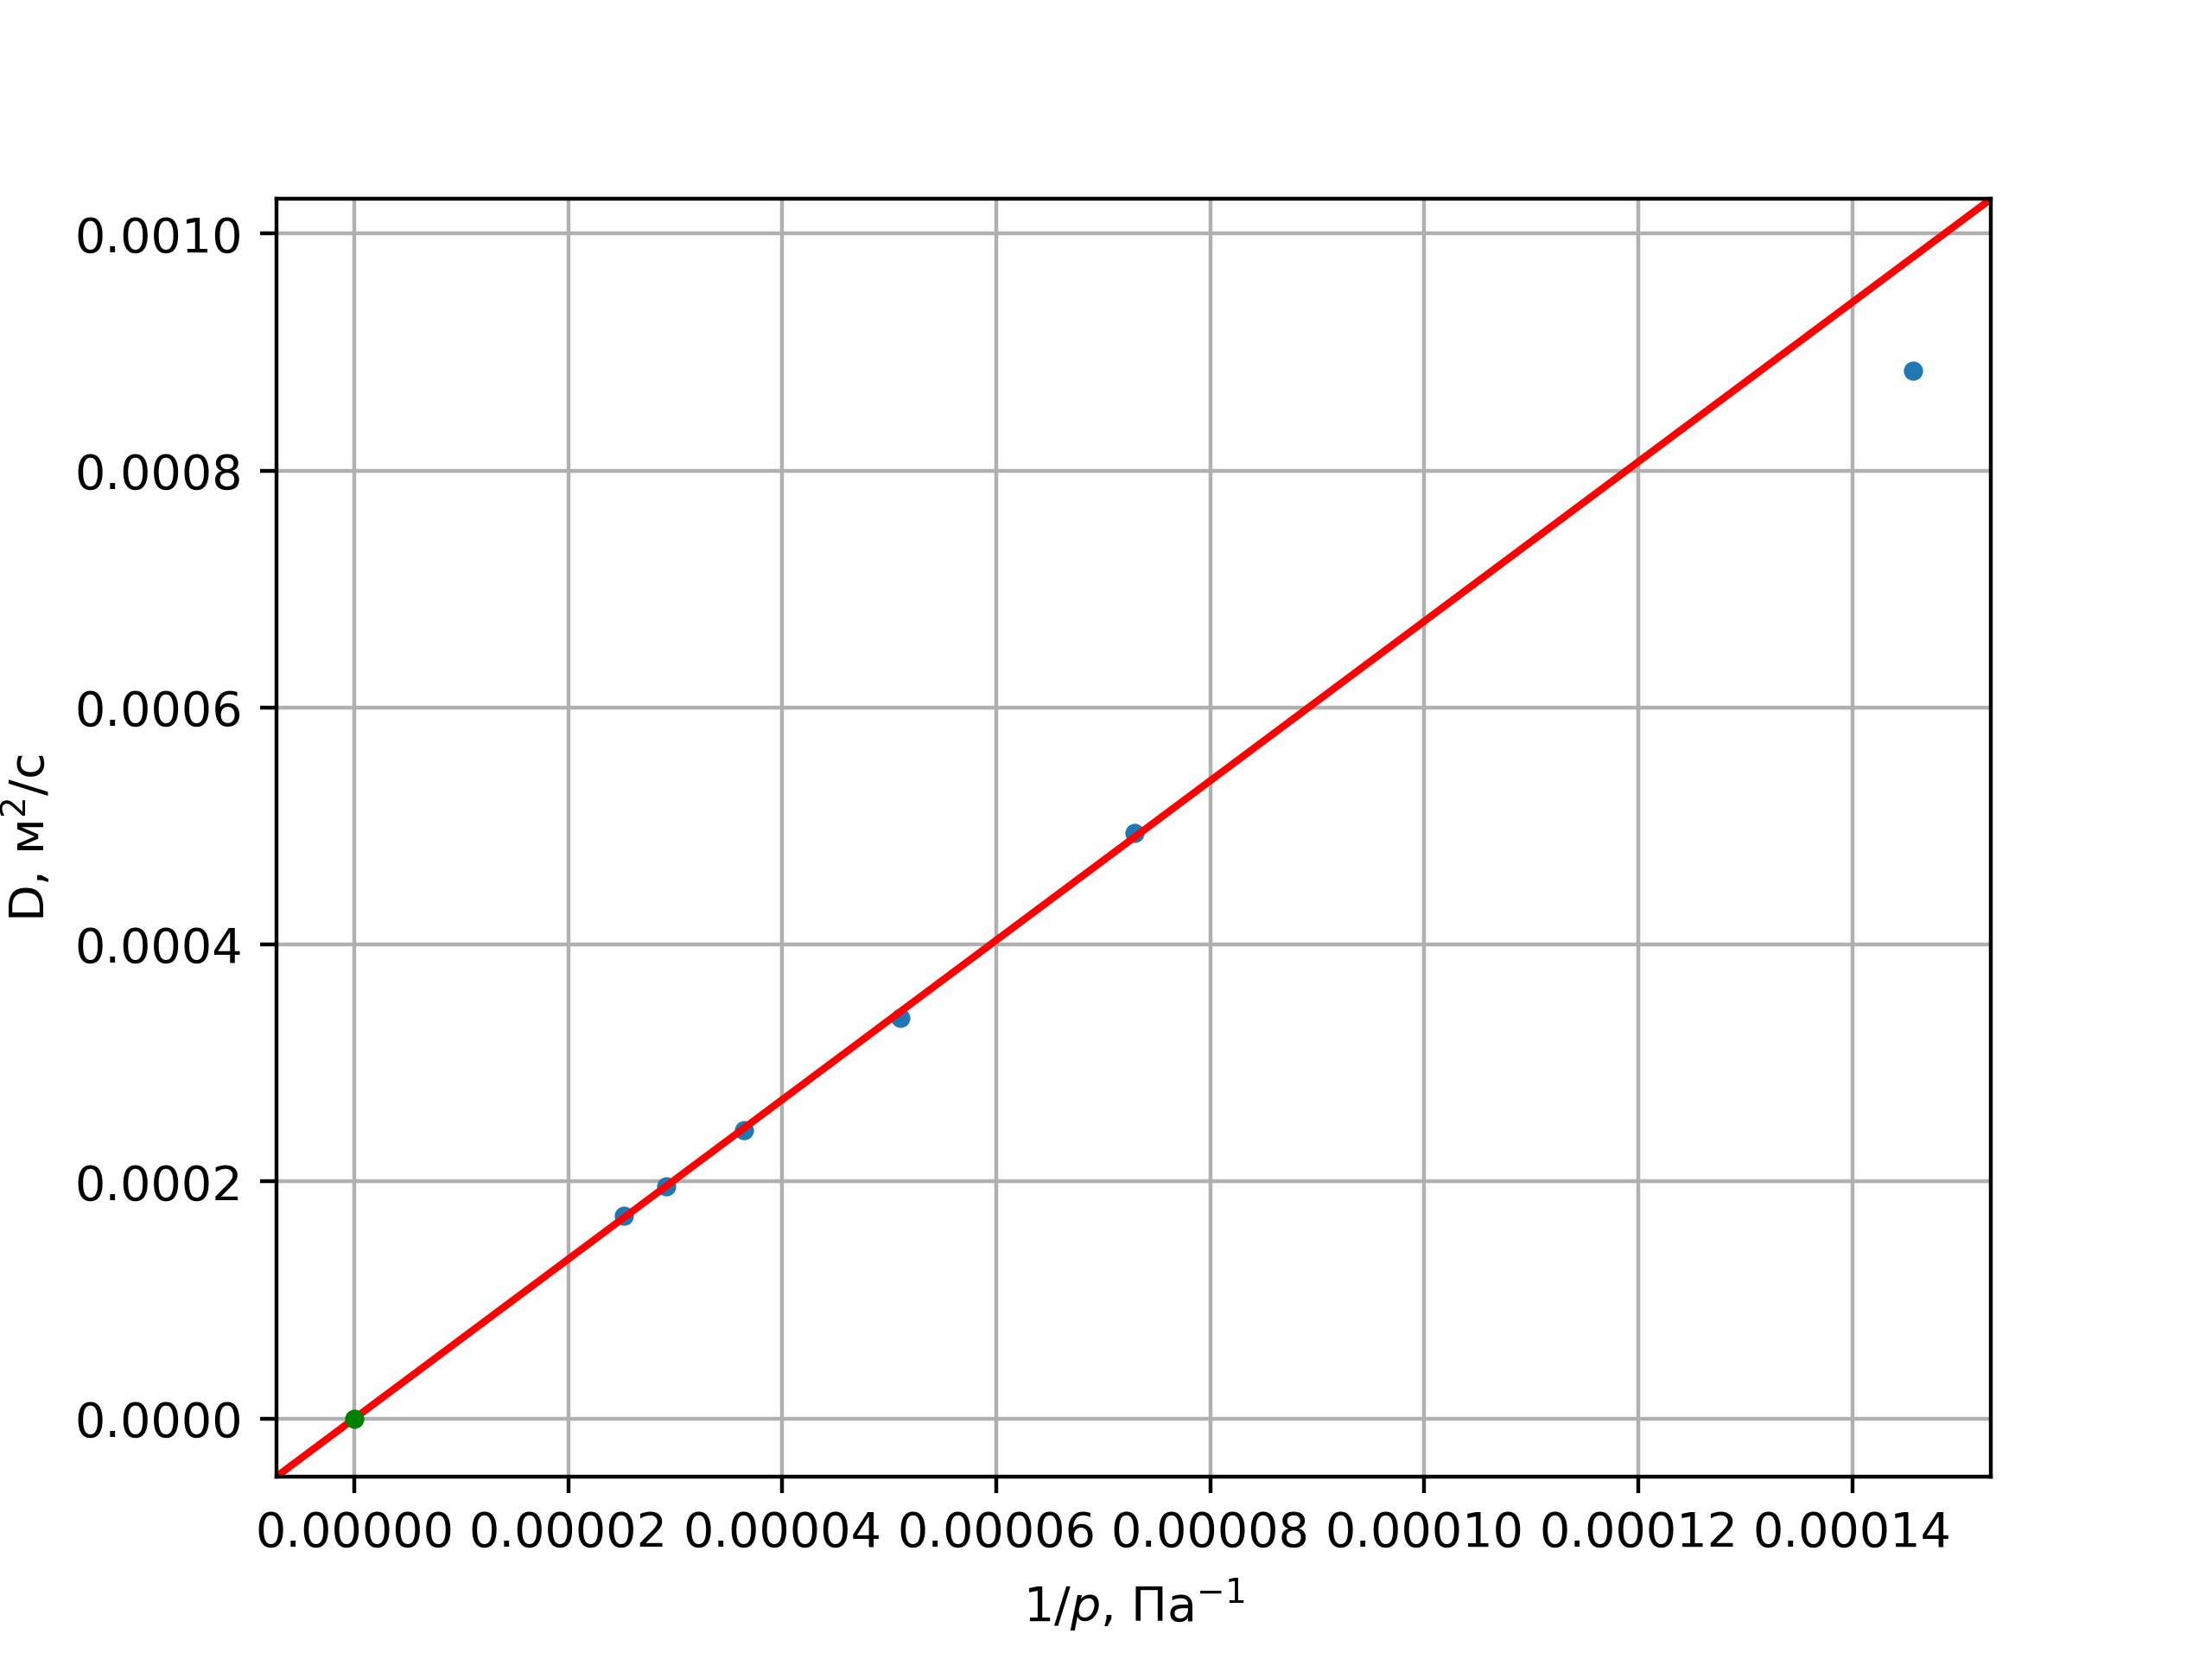
\includegraphics[width=0.8\linewidth]{img/total.png}
\end{figure}

\[k = 6{,}73\pm 0{,}03\,\text{Н}/\text{с}\]
\[D_0 = k / 101325\,\text{Па} = \left(6{,}64\pm 0{,}03\right)\cdot 10^{-5}\,\text{м}^2/\text{с}\]

При комнатной температуре
\[\lambda\approx 1\,\text{мкм}\]
\[\sigma\approx 2{,}5\cdot 10^{-19}\,\text{м}^2\]
